\documentclass[letterpaper]{article}
\usepackage{natbib,alifexi}
\usepackage[T1]{fontenc}
\usepackage{lmodern}
\usepackage[utf8]{inputenc}
\usepackage{abstract}
\usepackage{textcomp}
\usepackage{amsmath}
\usepackage{graphicx}
\usepackage{placeins}
\usepackage{titlesec}
\usepackage{algorithm}
\usepackage[noend]{algpseudocode}
\usepackage{url}

\makeatletter
\def\BState{\State\hskip-\ALG@thistlm}
\makeatother

\DeclareMathOperator*{\argmax}{arg\,max}
\DeclareMathOperator*{\argmin}{arg\,min}

\titlelabel{\thetitle.\quad}

\title{Study of various algorithms for identifying tonalities in music pieces, \\ proposal of different approaches for key retrieval \\ and their implementation in Clojure}
\author{Antoine Passemiers$$ \\
Promoter: Bernard Fortz\\
\mbox{}\\
$$Université Libre de Bruxelles \\
apassemi@ulb.ac.be}

\begin{document}
\maketitle

\renewcommand\bibname{References}        % Change the bib title
\renewcommand{\refname}{References}
\makeatletter
\renewcommand\@biblabel[1]{#1.  }
\makeatother

\setcounter{secnumdepth}{3}

\begin{abstract}
The project involves the discussion of different approaches to automated tonality retrieval from audio files,
the prototyping of these methods, a reflexion on their consistency with functional programming,
and the implementation of the most appropriate ones in Clojure.
State of the art comprises various maximum key-profile correlation (MKC) approaches and machine learning algorithms, and this
project implies to review all of them after implementing them in Python. Also, the second goal is to
assess the accuracy and speed of different MKC-based approaches in Clojure.
\end{abstract}

\section{Introduction}

The tone of a musical work is characterised by the set of sounds coming from a same diatonic scale.
Unlike scales, where musical notes follow each other in a contiguous manner, tones assemble notes that can be
disjoined or even overlapped \citep{AD}.
Therefore, our central concern is the analysis of polyphonic melodies, which constitute the overwhelming
majority of the modern musical works.\\

Key finding algorithms rely on spectral estimation and are expected to get a chroma vector as input. The chroma vector contains, for each musical note (the chromatic scale consists of twelve distinct notes), its corresponding strength. As a consequence, regardless of how we estimate the spectrum, this spectrum must be compacted in a vector of exactly twelve coefficients.\\

More specifically, we will give consideration to two types of tonality prediction methods:
those based on tone profiles, and those based on machine learning algorithms.
The former aims to integrate the acquired knowledge on the cognitive theory, whereas the latter
use statistical inference to extract the relevant information from the music tracks.
The cognitive-inspired approach used for identifying tones is partly dependent on the solution design suggested by S. Pauws \citep{SP}, and later by
Ibrahim Sha\textquotesingle ath for the software KeyFinder \citep{IS}. Also, some discrepancies between their solutions and our final implementation will be explained. \\

As regards the machine learning techniques, those presented from sections \ref{sssec:hmm} to \ref{sssec:iohmm}
are mainly linked to Hidden Markov Hodels and Neural Networks. The cross-validation of these models has been achieved by splitting
the database in a training set and a validation set. Being intended to remain brief, the present report focuses on the methodology used,
and short descriptions of the algorithms discussed, with emphasis on how the proposed solution differs from the other solutions. Finally, only the results of the MKC-based algorithms will be presented, since machine learning techniques did not provide satisfactory results.

\section{Theoretical considerations}

\subsection{Preprocessing}

The audio signal is first extracted from the WAV file, and then the average of its channels is calculated
if the file has been written in stereo. It is not required to take the pan into account given that mixing
channels in the temporal domain or in the spectral domain makes no difference, thanks to the property of linearity of the Fourier transform.
Steven W. Smith devoted a specific chapter of his book \textit{The Scientist and Engineer's Guide to Digital Signal Processing} to the properties of the Fourier transform, including the property of linearity \citep{PHD}. \\

Also, there is no indispensable need to consider the whole frequential bandwidth given that notes are mainly characterised 
by their fundamental frequency
and that the harmonics of the highest existing notes (high C or 1046 Hertz if we consider the vocal range, for example) are not relevant for estimating chromagrams, since the task does not consist in identifying the instruments.
The sampling rate is de facto resampled at a tenth of the standard sampling frequency (4410 Hz).
Although this substantial downsampling is likely to create aliasing effects (which can be simply avoided by 
applying a low-pass filter), no loss of accuracy has been pointed out during the evaluation phase.

\subsection{Spectral estimation}

There are two broad categories of spectral density estimation techniques: the parametric ones and the non-parametric ones \citep{MHH}. The techniques
of which we will be speaking are all non-parametric algorithms. More specifically, we are going to discuss methods based on the discrete-time Fourier transform (which are the most often used) and least-squares spectral estimation techniques. Fourier-based and least-squares methods have achieved comparable results in terms of accuracy.

\subsubsection{Direct Spectral Kernel Transform (DSKT)}

This algorithm has been proposed by Ibrahim Sha\textquotesingle ath, and appeares to be a fast and efficient approximation of the Constant-Q Transform implementation as described by Brown and Puckette \citep{CQT}.
The data samples are first multiplied by a Blackman window to avoid spectral distortions. Then the spectrum is approximated by the Fast Fourier Transform.
The spectral kernels are computed a posteriori by applying cosine windows in the spectral domain, centered on the frequencies of interest. The advantage is that each window can be pre-calculated and reused each time the DSKT needs to be applied. The particularity of the DSKT is that the bandwidth around each frequency of interest is constant, and determined by the parameter Q. To calculate the bounds of a kernel of central frequency $ f_k $, we refer to the following formulas:

\begin{align}
l_k  = (1 - \frac{Q}{2}) \cdot \frac{f_k \cdot N}{s}
\end{align}

\begin{align}
r_k  = (1 + \frac{Q}{2}) \cdot \frac{f_k \cdot N}{s}
\end{align}

\noindent as established by Sha\textquotesingle ath, where $N$ is the resolution of the Fourier transform, and $s$ is the sampling rate (after downsampling).

\subsubsection{Van\'{\i}\v{c}ek least-squares spectral estimation}

It is also possible to estimate the spectrum using dedicated regression techniques. We will give focus on the most popular of them:
the Van\'{\i}\v{c}ek method and the Lomb-Scargle method. A spectrum approximated by one of the latter is called a periodogram.
Handling missing data samples and non-uniform data is a rationale for the Van\'{\i}\v{c}ek method, since it has been developped in the fields of
geology and astrophysics, where data are not received at regular intervals. Furthermore, unlike the Fast Fourier Transform which has a
variable spectral resolution (depending on the size of the observation window), the least-squares methods output periodograms of a size
that is equal to the number of trial frequencies. Theoretically, this is an interesting feature since we only need to focus on the musical notes that fall in the spectral bandwidth of interest. This can not be achieved using FFT-based algorithms. The only constraint is that the number of data samples must be higher than the number of trial frequencies.\\

According to the Van\'{\i}\v{c}ek method, the signal is assumed to be a linear combination of sine and cosine waves, with given frequencies of interest.
The coefficients of the linear combination are stored in a vector $c$, and the signal is assumed to be $f \approx \phi.c$. 
Each column of the matrix $\phi$ contains the data samples of the sine and cosine waves of a particular trial frequency.
Finally, the coefficients are derived from the least-squares method, and given by the equation \ref{fig:linreg} \citep{PS}.

\begin{align}
\hat{c} = (\phi^{T} \phi)^{-1} \phi^{T} f
\label{fig:linreg}
\end{align}

This method is very similar to the matching pursuit algorithm. The idea of the matching pursuit is to represent the signal as a finite linear combination of given
functions, referred as atoms. At iteration k, the atom that minimizes the least squares residuals is weighted and then subtracted from 
the remainder of the signal. Once every trial frequencies has been treated, the weights are grouped into a single spectral estimation vector.

\subsubsection{Lomb-Scargle least-squares spectral estimation}

As we can see from formula \ref{fig:linreg}, the Van\'{\i}\v{c}ek\textquotesingle s strategy is lacking consideration for the phases of the trial sine waves.
The consequence is that sinusoids of a same frequency can be highly correlated. The new approach requires that each pair of sinusoids at a given frequency
is mutually orthogonal at each time $t_{j}$. Let\textquotesingle s set $\tau$ the phase change to apply to both the sine wave and the cosine wave to make
them mutually orthogonal for each data sample. Luckily, this phase change can be pre-calculated and is given by the equation \ref{fig:phases} \citep{LS}.

\begin{align}
\tan 2\pi f \tau = \frac{\sum\limits_{j=1} \sin 2\pi f t_{j}}{\sum\limits_{j=1} \cos 2\pi f t_{j}}
\label{fig:phases}
\end{align}

Contrary to the formula \ref{fig:linreg}, which consider all the trial frequencies at once, Lomb\textquotesingle s approach suggests to fit the signal to a single sinusoid at a time, and consider the rest of the spectrum as being random noise. This process is repeated progressively for each trial frequency. The weight $R(f)$ of each trial frequency is then grouped together with the others, resulting in a periodogram. $R(f)$ is a linear combination of
the signal-cosine wave correlation and the signal-sine wave correlation, and results in the following equation:

\begin{align}
\Delta R(f) = \frac{(YC)^{2}}{CC} 
+ \frac{(YS)^{2}}{SS}
\label{fig:ccss}
\end{align}

Also, the power of the cosine wave and the sine wave are different for the same trial frequency. To rebalance the previous equation, the terms $(YC)^2$ and $(YS)^2$ are divided respectively by the energy of the cosine wave (CC) and the energy of the sine wave (SS).
Fortunately, CC and SS can be pre-calculated as well, since the trial frequencies don\textquotesingle t change from a music track to another. The energy is simply computed as a regular sum of squares:

\begin{align}
CC = \sum\limits_{j=1} \cos^{2} 2\pi f (t_{j} - \tau)
\label{fig:cc}
\end{align}

\begin{align}
SS = \sum\limits_{j=1} \sin^{2} 2\pi f (t_{j} - \tau)
\label{fig:ss}
\end{align}

YC and YS terms measure the correlation between the data samples and, respectively, a cosine wave and a sine wave of frequency $f$. Once again, we are
benefitting from the fact that the sine and cosine waves can be pre-calculated and reused for each transform.

\begin{align}
YC = \sum\limits_{j=1} y_{j}\cos 2\pi f (t_{j} - \tau)
\end{align}

\begin{align}
YS = \sum\limits_{j=1} y_{j}\sin 2\pi f (t_{j} - \tau)
\end{align}

Therefore, the only remaining operations that cannot be processed at compile-time are the scalar products of the sinusoids and the current chunk, which
reduces drastically the number of required operations to estimate the spectrum.\\

Contrarily to Fourier-based
estimators, the periodogram seems to suffer from spectral imbalance: this phenomenon is illustrated in the appendix B. When the periodogram consists of several peaks, the highest peak will always be relatively much higher than the others, compared to what we can get with the Fourier transform.\\

This report proposes a simple solution to this issue. The idea consists in enriching the spectrum with musical notes located in a different chunk of data samples. In fact, an heptatonic musical scale is characterized by a set of seven notes, but it is
not common to meet them all at the same moment. Because it is not possible to make a spectral analysis of contiguous notes, the alternative is to overlay them.
Let\textquotesingle s illustrate this effect. In figure \ref{fig:frame1}, 
we can observe one dominant peak from the Lomb-Scargle periodogram. In figure \ref{fig:frame2} (representing the next frame), we can clearly distinguish two peaks. By summing the two frames, a complex shape appears, which highlights the non-linearity of the Lomb-Scargle periodogram.\\

\subsubsection{Other spectral estimation techniques}

Various methods are not discussed in this report, such as the Pisarenko Harmonic Decomposition (PHD), the MUSIC algorithm or the EigenVector Method. All of them are summarized in the article of Al-Azzo and Al-Sabaawi and compared for the estimation of direction-of-arrival of ultrasonic signals \citep{MA}. They may be considered in a future work and compared to the Lomb-Scargle method in terms of accuracy.

\subsection{Key identification}

Once the spectrum is approximated, it is reshaped into a chroma vector of twelve coefficients. In the frameworf of the algorithms assessment, it has been found that 6 octaves are sufficient to evaluate the spectrum: the addition of a seventh octave does not improve the accuracy of the predictions. With this knowledge, the spectrum - which has a resolution of 72 coefficients is reshaped into a matrix $M_{i, j}$ of dimension $(6 \times 12)$. Finally, the chroma vector is obtained by formalising the method developed by Sha\textquotesingle ath:

\begin{align}
C_{i} = p * \max_{j} M_{i, j} + (1 - p) * \sum_{j} M_{i, j}
\label{chroma}
\end{align}

where p is a parameter determined during the evaluation / validation of the whole system.
The last step consists in identifying the tonality locally,
on the basis of this single chroma vector. We are going to discuss different methods, the first one relies on the Maximum Key-Profile Correlation (MKC),
while the others are based on machine learning algorithms.

\subsubsection{Cognitive models}

This solution relies on the Maximum Key-Profile Correlation approach: the idea is to compare the chroma vector (obtained from the previous step) to
tone profiles that have been pre-defined by experts. The profile that maximizes the correlation with the chroma vector indicates which key is the most probable
for the current chunk of data samples \citep{AT}. This method is the ths most commonly accepted, and described also by S. Pauws \citep{SP}. Both of them use profiles coming from the experience conducting par Carol L. Krumhansl and Lola L. Cuddy on tonal hierarchies in music and their perception by man.\\

In short, the experience was conducted as follows: incomplete scales were played in front of subjects, followed by additional notes that the latter were asked to rate according to their capacity to match scales. The scores obtained from this study were grouped into two chromagrams, showed by the figure \ref{krumhansl}. \\

\begin{figure}
\begin{center}
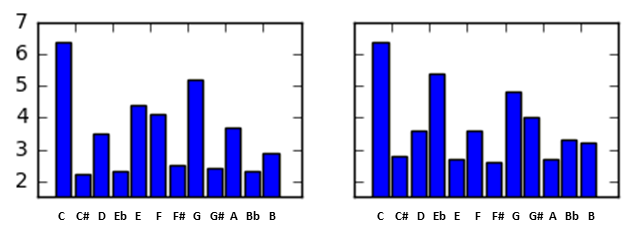
\includegraphics[width=3.1in,angle=0]{imgs/Krumhansl.png}
\caption{Krumhansl tone profiles representing the C major and the C minor scales, respectively.}
\label{krumhansl}
\end{center}
\end{figure}

Although these two tone profiles provide satisfactory results when the spectrum is approximated by the Constant-Q transform, they are no longer valid 
when the Lomb-Scargle method is used, since it was observed that periodograms consist of coefficients that are broadly distributed more evenly. This distribution has to be reflected in the tone profiles and that is why the algorithm has been evaluated a sufficient number of times, until the tone profiles
provide satisfying results. The adjusted tone profiles are shown in the figure \ref{profiles}.

\begin{figure}
\begin{center}
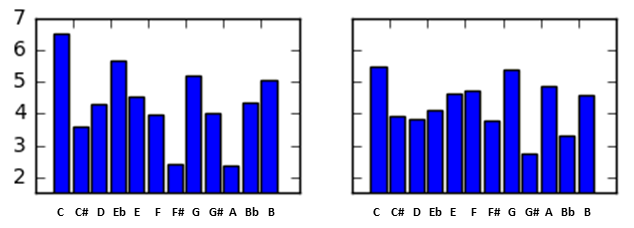
\includegraphics[width=3.1in,angle=0]{imgs/Custom.png}
\caption{Best tone profiles, determined empirically and adjusted for the Lomb-Scargle periodogram.}
\label{profiles}
\end{center}
\end{figure}

\subsubsection{Spiral Array CEG Algorithm}

The Spiral Array Center of Effect Generator solution has been proposed by Elaine Chew \citep{SPIRAL}, and solves the problem for both spectral estimation and key retrieval, by taking the geometric arrangement of notes into consideration.
In a manner similar to the DSKT, the spectrum is divided into various pitch frequency bands, centered on the frequencies of interest. Then a heuristic peak detection algorithm is employed for each frequency band, where 
at most one local maximum may be identified. The chroma vector is obtained by mapping the peak strengths using the formula \ref{chroma} with $p = 0$, and by normalizing the resulting vector along the time axis and then by normalizing the vector itself.\\

The spiral array consists, in the three-dimensional space, of a sequence of twelve pitch classes arranged on a spiral, where adjacent pitch class points are related by intervals of five semi-tones, and vertical neighbors are related by intervals of four semi-tones. Major and minor keys are described as linear combinations of the twelve pitch class points, and arranged inside the spiral beforehand. The key retrieval algorithm is explained as follows: the coefficients of each chroma vector are re-used as weights for linear combinations of the pitch class points, which results in a single point in the 3D space. This process is repeated cumulatively on a frame basis, and finally a nearest-neighbor search is employed to find the closest pitch class point to the previous single point \citep{MIDI}.\\

In the context of our work, we simply used the euclidean distance as a criterion for the nearest-neighbor search. Unfortunately, the Spiral Array CEG algorithm did not provide as good results as the MKC-oriented techniques. Chew described many other ways to represent pitch classes in her book \textit{Mathematical and Computational Modeling of Tonality : Theory and Applications} \citep{CHEW}, such as the Krumhansl\textquotesingle s pitch cone and the Lerdahl\textquotesingle s pitch cone, which may be considered in a future work.

\subsubsection{Hidden Markov Models (HMM)}
\label{sssec:hmm}

Hidden Markov Models are discrete state machines that represent multivariate series by their distributions and by
the transition probabilities between their states. Their states are called “hidden” because they are not observed directly,
but can be inferred from the observation sequence using a parameter estimation method (such as the expectation-maximization algorithm
or the Viterbi algorithm). Each hidden state distinguishes itself by its emission probabilities (or emission probability density function).
Unlike more popular machine learning models such as neural networks or support vector machines (SVM), Hidden Markov Models are capable of
processing input sequences of variable length. This characteristic is substantial given that music tracks are of variable length by nature\citep{DR}. \\

The old-fashioned way to classify keys using HMMs consists of training a HMM for each distinct music key, and to predict the most probable 
key of an unlabelled music track by looking for the HMM that maximizes the probability of occurence.  \\

According to J. Peeters \citep{JP}, if the training set is unbalanced (which is also the case in the present study), overfitting may occur on the specificities
of each music track. The solution is to fit two mode-specific HMMs: one for the C major mode and one for the C minor mode. In order to do this, every chroma vector is circularly shifted of the number of semi-tones separating the ground-truth key and the root-node of C. Next, for both C major and C minor HMMs, a circular shift is applied on the mean vectors and covariance matrices of each hidden state to map them to a specific scale. Finally, the new HMMs are used as regular HMMs for classification.\\

In the article of Papadopoulos and Peeters \citep{PP}, the sequence of hidden states is inferred using the Viterbi decoding algorithm. The most probable sequence of hidden states gives the succession of local keys. It is then possible to segment a same music track in different keys if the latter contains multiple tonalities.

\subsubsection{Feedforward neural networks}

Neural networks have already delivered good results for classifying chords inside a same piece of music \citep{JO}.
The problem is that chroma vectors are too short to feed a neural network if the latter has to discriminate between 24 classes. In the study of Osmalskyj, 
they are very few types of chords to classify, which eases the prediction task. Furthermore, neural networks cannot learn the variations of the pitch distribution over time, on the only basis of the key: the song must be labelled on frame basis. The solution is to take the time factor into account, as described in the next sub-section.

\subsubsection{Input-Output Hidden Markov Models (IO-HMM)}
\label{sssec:iohmm}

An IOHMM is a Markov model where each hidden state emitting probability distribution is actually a conditionnal probability distribution, inferred using a gradient descent algorithm, as well as the state transition probability distribution \citep{YB}. This model has already been discussed in the framework of other tasks linked to  music pieces, such as chord predictions. \\

The main deficiency of the standard HMM is that it has no discriminative capabilities: if one of the keys appears to be more frequent in the database or
if it seems to be easily explained by the HMM, the latter will present high risks of predicting the same key every time, regardless of the
input sequence. On the other hand, feedforward neural networks have the defect that they are not suited for temporal data, since they must 
process feature vectors of fixed size. \\

The Input-Output Hidden Markov Model is well suited for our task because it is affected by none of these deficiencies.
However, we could not achieve good results with this model, due to overfitting problems. In a future work, it would be profitable to get a bigger and better balanced dataset.

\subsubsection{Markov Chains of Local Key Predictions}

Because a MKC algorithm has been employed to design the final Clojure architecture, we had to consider the factor of time. This report proposes a new approach to achieve this: view frame-based predictions as chords and taking only the probabilities of transition between chords into account. From now on, we call a frame-based prediction a sample. In a markovian process, all the information required to model the probability of realization of a future sequence is contained in the sample located at present time. As a consequence, we can model the probability of realization of the samples sequence as the product of the transition probabilties in all pairs of adjacent samples. For numerical stability purposes (because the sequence can be very long), the product of probabilities is replaced with a sum of log-probabilities. We set $T$ the number of samples and $P[i=s_t, j=s_{t-1} | k = c]$ the probability of transition from sample $s_{t-1}$ to sample $s_{t}$, where $c \in \{0, ..., 24\}$ is a global key. The most probable key is then given by:

\begin{align}
\hat{c} = \argmax_c \sum_{t=2}^{T} \log_2 P[i=s_{t-1}, j=s_{t} | k = c]
\label{logproba}
\end{align}

This suggests that we determine a transition probability matrix for each $c \in \{0, ..., 24\}$, but it is preferable to prevent overfitting problems by adapting Peeter\textquotesingle s solution (as described in sub-section \ref{sssec:hmm}) to Markov chains. Instead, a single transition probability matrix is constructed for all keys. This implies that sample sequences are viewed as homogeneous Markov chains \citep{AUTOMATA}, and the process will be described with more details in sub-section \ref{sssec:A}.

\section{Methodology}


\subsection{Clojure implementation}

Clojure is a dynamic and functional programming language based on the Java Virtual Machine, suited for quickly designing multithreaded programs,
and featuring a full range of immutable and/or persistent data structures. It benefits from both the advantages of compiled languages and dynamic typed
languages, which allows us to write optimized code in a small amount of time, using a fancy syntax. However, although Java libraries can be imported into the Clojure environnement, there is a comparatively small number of libraries that are natively implemented in Clojure. In our case, the majority of the functionalities
are implemented exclusively for the project. Because the Clojure machine learning libraries are at their first steps, we are not using any machine learning 
technique in the design of the final algorithms.\\

The objective of this section is to describe the functional solution design for Clojure, and compare the Lomb-Scargle periodogram and the direct spectral kernel
transform in terms of speed and accuracy. Finally, we will insist on the choices that differ from state of the art from a theoretical point of view.\\

In order to test the numerous features of the project, unit tests have been implemented. In addition, Tufte (a Clojure profiling library) has been used to assess the performance of the various parts of the system. For all the performance-critical areas of the code, we will see the different measures shown by Tufte.\\

\subsection{Solution design}

\begin{figure}[h!]
\begin{center}
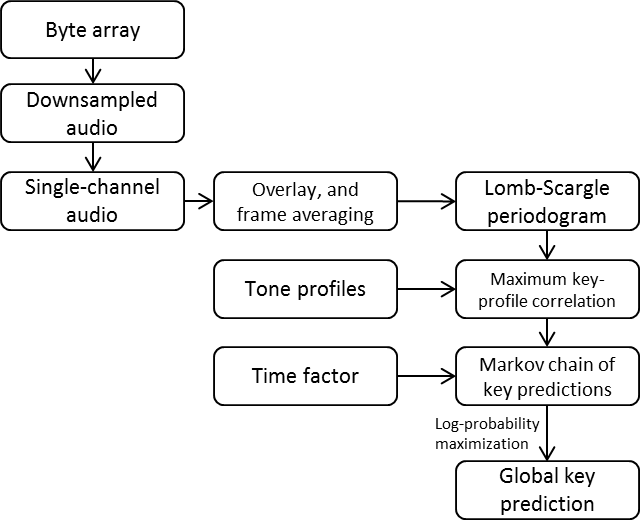
\includegraphics[width=3.1in,angle=0]{imgs/flowChart.png}
\caption{Flowchart: solution design}
\label{fig3}
\end{center}
\end{figure}

\subsubsection{Downsampling and channel averaging}

Since downsampling without filtering has no significative impact on the accuracy, a dedicated WAV file reader has been designed to convert a byte stream directly
at the target sampling rate. This is to process far less data samples, thus helping to gain speed. In addition, the downsampled signal is then returned as
a lazy Clojure sequence, ensuring that we don\textquotesingle t evaluate data samples we are not using in the end.
The next step consists of, in the case of a multi-channel audio, averaging the multiple channels. The result of this operation yields a lazy sequence, following
the same logic.

\subsubsection{Lomb-Scargle periodogram}

Considering the fact that spectral estimation remains the performance-critical area of the code, regardless of the technique used, type hints have been added to the functions and var names involved. This is to help the compiler infer the type of return values at compile-time.
At this stage of the code, we are only handling primitives and \textit{clojure.lang.LazySeq} objects (Clojure lazy sequences).\\

We know from equations \ref{fig:cc} and \ref{fig:ss} that the terms CC and SS can be pre-calculated. As a consequence, they are computed at compile-time,
for every trial frequency, and can be reused for each spectral estimation. For this reason, a vector of \textit{PreprocessedWaveforms} objects has been statically defined. A \textit{PreprocessedWaveforms}
type regroups a specific trial frequency, the associated phase change, sine wave and cosine wave, and the corresponding CC and SS terms.\\

\subsubsection{Direct spectral kernel transform}

For the purpose of this work, the iterative radix-2 fast Fourier transform has been reimplemented according to the functional paradigm. An inplace version of the FFT is described in \textit{Introduction to algorithms} \citep{FFT}, and its pseudo-code is organized as given in appendix A. A Clojure complex number type has been defined, as well as common operators such as addition, subtraction, mutiplication have been redefined. \\

Some adjustments have been performed to implement the iterative FFT in a Clojure fashion. Java arrays have been used to store the spectral coefficients, but without relying on any temporary variable. To accomplish this, the first loop (line 4) and second loop (line 7) have been replaced by using the \textit{mapv} macro. The problem was that the complex number $\omega$ is changing state at each iteration of the third loop. In place of mutating $\omega$, the latter is returned by an anonymous function at every iteration $j$ and used as an input at iteration $j + 1$. This process is allowed to be very efficient in Clojure, and shown by the following picture:

\FloatBarrier

\begin{figure}[h!]
\begin{center}
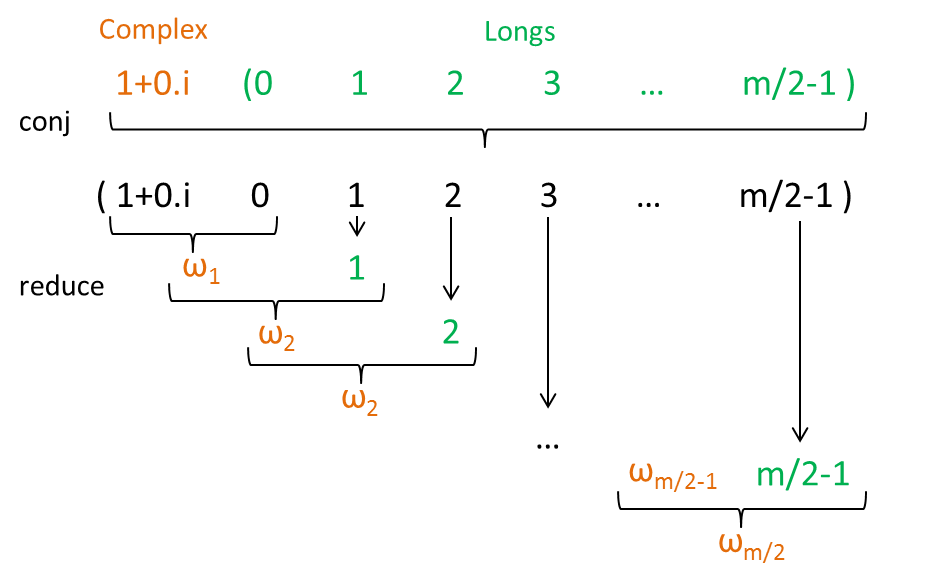
\includegraphics[width=3.1in,angle=0]{imgs/reduceconj.png}
\caption{Dealing with the state of $\omega$ in the inplace FFT}
\label{fig3}
\end{center}
\end{figure}

\FloatBarrier

Type hints and Java data structures have been employed according to the Java interop guide of Clojure \citep{CL}.

\subsubsection{Markov Chains of Frame-based Predictions}
\label{sssec:A}

We set $A_{i, j}$ the element $(i, j)$ of the transition probability matrix. The latter has been determined empirically during the evaluation process, by counting the occurences of each possible transition:

\begin{align}
A_{i, j} = \sum_f \sum_{t=2}^{T_f} \big[ i=rotate(s_{t-1}, k_f) \wedge j=rotate(s_t, k_f) \big]
\label{MIJ}
\end{align}

$T_f$ is the length of the samples sequence extracted from file $f$ and $k_f$ is the ground-truth label corresponding to file $f$.
Despite the fact that the probability matrix has been calibrated on the C major key, it is possible to get the 23 other keys by rotating this matrix along its two axes.
This is made artificially by rotating the indices while accessing the matrix elements.

\begin{align}
rotate(s_t, k_f) = (s_t + 24 - k_f) \mod 24
\label{rotate}
\end{align}


Once the matrix is built, the prediction process is such that the most probable key is the one that maximizes the product of the transition probabilities between adjacent samples, 
where the samples are rotated for each $c \in \{0, ..., 24\}$ to simulate the existence of one transition probability matrix per key.

\begin{align}
\hat{c} = \argmax_c \sum_{t=2}^{T} \log_2 A_{rotate(s_{t-1}, c), rotate(s_{t}, c)}
\label{logprobaclojure}
\end{align}

The transition probability matrix has been stored statically as a matrix object from the \textit{core.matrix} API. \textit{core.matrix} is a useful library for handling multi-dimensional arrays and applying efficient matrix operations. The transition probability matrix is shown in appendix C.

\subsubsection{Datasets}

The database consists of 415 music tracks recorded in WAV format, 44100 Hz stereo, associated with annotated keys (determined beforehand).
All keys have been determined
by experts and have been made available by Ibrahim Shat\textquotesingle ath as part of its work. For evaluating algorithms based on MKC,
all the tracks have been used to tune the parameters to their best value. The latter consist of: the major and minor tone profile coefficients,
the size of the sliding window, the frequency range of the spectrum, the parameter $p$, and the transition probabilities for modelling the Markov chains of frame-based predictions. For evaluating machine learning techniques,
the dataset has been split into a training set of 138 music tracks and a validation set of 277 tracks.

\subsubsection{Evaluation}

In the framework of this study, we consider only the twelve heptatonic major scales and the twelve heptatonic minor scales.
Two different metrics are used to evaluate the accuracy of the algorithms:
the raw accuracy (the ratio between the number of correct predictions to the number of analyzed files) and the metric invented for the Music Information Retrieval Evaluation eXchange \citep{MIREX}.
The MIREX metric is a weighted sum of the number of correct predictions (C), the number of predictions that are out by a fifth (F), the number of predicted scales that are parallel to the correct ones (P), and the number of predicted scales
that are relative to the correct ones (R). The index is then given by: \\

\noindent $ MIREX = (C + \frac{1}{2}.F + \frac{3}{10}.R + \frac{1}{5}.P) / TOTAL $ \\

Since the Markov chain classifier necessitates a transition probability matrix of 24 x 24 = 576 elements, it introduces a risk of overfitting the database. To ensure this is not the case, the dataset has been split into a group of 207 files (used for building the matrix) and a group of 208 files for evaluating the algorithm. An improvement of 3 \% in accuracy has been noted, compared to a naïve method such as taking the most frequent frame-based prediction. This validates the gain of accuracy the Markov chain provides. Lastly, the whole dataset has been re-used to fit the final transition probability matrix.

\section{Results}

It comes out of this study that the results are much better if we set the parameter $p$ to zero, regardless of the spectral estimation technique used.
The optimal tone profile coefficients are shown in figure \ref{profiles}. For both DSKT and LS methods, a window size of 4096 samples has provided good results. For the LS periodogram specifically, adjacent frames have been overlayed, which results in an overlap of 4096 samples.
Considering a frequency band bounded by $G\#1$ and $G\#6$ seems to be sufficient to cover the whole spectrum: no significant accuracy improvement has been noticed while increasing the frequency range.\\

Despite the fact the Lomb-Scargle estimation method is well-suited for processing frames that have arbitrary sizes, we could not benefit from this feature since beat detection provided no greater accuracy. In a future work, it would be preferable to evaluate the Lomb-Scargle technique by combining it with state-of-the-art tick detection algorithms.

\begin{table}
\center{
\begin{tabular}{|c|c|c|c|}\hline
Method & Accuracy & MIREX & $\tau$ \\ \hline\hline
DSKT (Java) & - & - & 94,64 $\mu$s \\
DSKT (Clojure) & 47,2\% & 55,5\% & 9,4 ms \\
LS (Clojure) & 47,9\% & 57,7\% & - \\
DSKT (Python) & 54,2\% & - & - \\
LS (Python) & - & - & - \\
\hline
\end{tabular}
}
\vskip 0.25cm
\caption{Accuracy assessment, according to the raw accuracy and the MIREX index}
\end{table}

TODO\\
DSK : 25 min 40 -> 3,75 seconds / file     | 194, 59, 10, 8, 140 \\
LS : 1 hour 30 min -> 13,13 seconds / file | 197, 70, 10, 11, 123 \\

\footnotesize
\bibliographystyle{apalike}
\bibliography{thesis}

\newpage

\section{Appendices}

\subsection{Appendix A - Inplace radix-2 FFT pseudo-code}

\begin{algorithm}
\caption{Iterative radix-2 FFT}\label{fft}
\begin{algorithmic}[1]
\Procedure{FFT}{a}
\State $BIT-REVERSE-COPY(a, A)$
\State $n \gets a.length$
\For{$(s \gets i) \text{ to } log_2(n)$}
	\State $m \gets 2^{s}$
	\State $\omega_m \gets e^{2\pi i / m} $
	\For{$(k\gets 0) \text{ to } n - 1 \text{ by } m$}
		\State $\omega \gets 1$
		\For{$(j \gets 0) \text{ to } m/2 - 1$}
			\State $t \gets \omega \cdot A[k + j + m/2]$
			\State $u \gets A[k + j]$
			\State $A[k + j] \gets u + t$
			\State $A[k + j + m/2] \gets u - t$
			\State $\omega \gets \omega \cdot \omega_m$
		\EndFor
	\EndFor
\EndFor
\EndProcedure
\end{algorithmic}
\end{algorithm}

\subsection{Appendix B - plots}

Due to the lack of linearity of the Lomb-Scargle periodogram, counter-intuitive effects seem to appear while plotting the periodograms. Indeed the different pitch strengths don\textquotesingle t have the same proportions between them, compared to the spectrum estimated with the Fast Fourier Transform.

\begin{figure}[h!]
\begin{center}
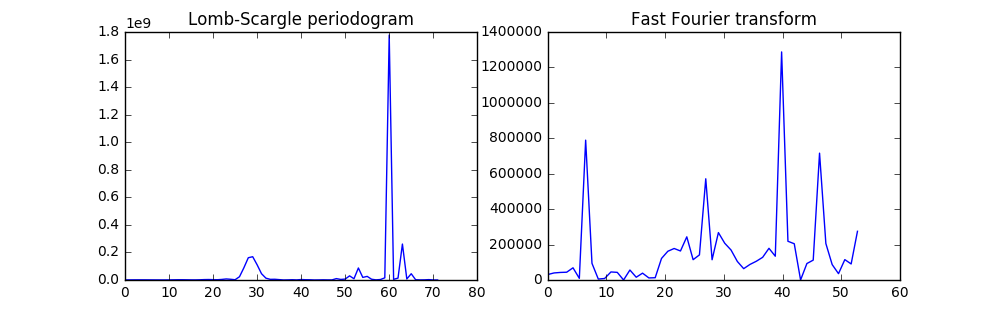
\includegraphics[width=3.1in,angle=0]{imgs/1frame.png}
\caption{Dreadlock holiday - 10cc, frame located at 2 min 44,17 s}
\label{fig:frame1}
\end{center}
\end{figure}

\begin{figure}[h!]
\begin{center}
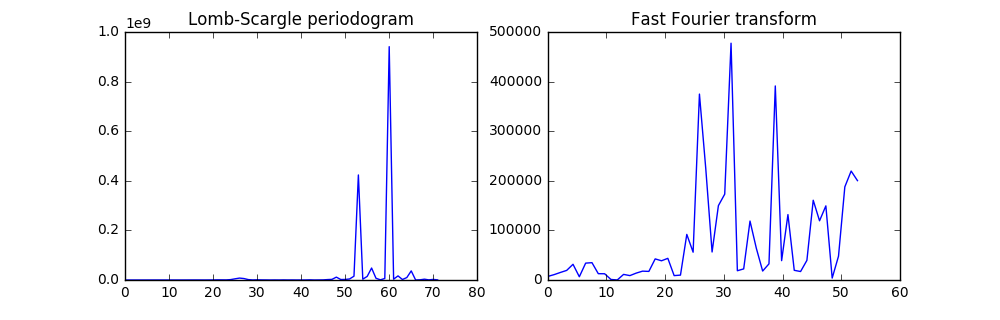
\includegraphics[width=3.1in,angle=0]{imgs/2frame.png}
\caption{Dreadlock holiday - 10cc, frame located at 2 min 44,27 s}
\label{fig:frame2}
\end{center}
\end{figure}

After summing the two frames in the temporal domain, we can observe new peaks appearing in the Lomb-Scargle periodogram, while the resulting Fourier transform shows a linear combination of the two first FFTs. This is shown in figure \ref{fig:frame1and2}.

\begin{figure}[h!]
\begin{center}
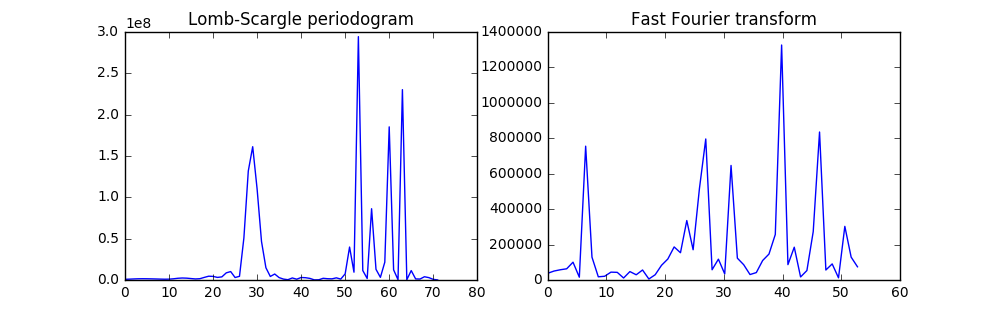
\includegraphics[width=3.1in,angle=0]{imgs/2frames.png}
\caption{Dreadlock holiday - 10cc, sum of the frames located at 2 min 44,17 s and 2 min 44,27 s}
\label{fig:frame1and2}
\end{center}
\end{figure}

\subsection{Appendix C - transition probability matrix}

\begin{figure}[h!]
\begin{center}
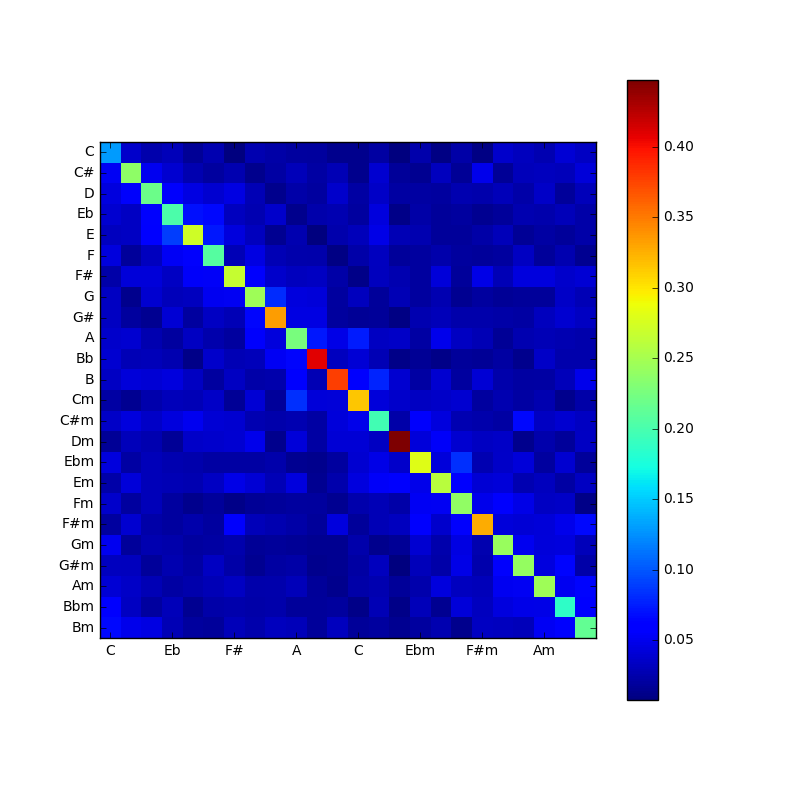
\includegraphics[width=3.1in,angle=0]{imgs/probs.png}
\caption{Transition probability matrix inferred from the 415 files of the database}
\label{}
\end{center}
\end{figure}

\subsection{Appendix D - Accuracy assessment according to the frame size}

\begin{table}
\center{
\begin{tabular}{|c|c|c|}\hline
Lomb-Scargle + MKC & Accuracy & MIREX \\ \hline\hline
4096 samples & 30,7\%  & - \\
8192 samples & 37,1\% & 48,9\% \\
12288 samples & 35,9\% & 48,0\% \\
16384 samples & 35,8\% & 48,9\% \\
\hline
\end{tabular}
}
\vskip 0.25cm
\caption{Scores obtained using Lomb-Scargle and a Maximum Key-profile Correlation approach, without any overlay and
without taking the temporal aspect into account.}
\end{table}

\end{document}